% Defence talk for the master thesis. Built on the Metropolis theme (see
% demo.tex for the theme's own examples). Figures are shared with the report:
% the TikZ files in ../pics are input as they are, with their thesis captions
% hidden, so the slides and the report always show the same drawing.
%
% Build from this folder:  tectonic -X compile defence.tex
\documentclass[10pt,aspectratio=169]{beamer}

\usetheme[progressbar=frametitle,sectionpage=none,numbering=fraction]{metropolis}
\usepackage{appendixnumberbeamer}

\usepackage{booktabs}
\usepackage{tabularx}
\usepackage{adjustbox}
\usepackage{tikz}
\usetikzlibrary{arrows.meta,positioning,shapes.geometric,fit,calc}

\usepackage[backend=bibtex,style=authoryear,maxcitenames=2,
            doi=false,isbn=false,url=false,eprint=false]{biblatex}
\addbibresource{../bibs/litDB.bib}
\renewcommand*{\bibfont}{\scriptsize}

\graphicspath{{../pics/}{figs/}}

\newcommand{\code}[1]{\texttt{\detokenize{#1}}}

% \thesisfig[max height]{path}: input a figure file from the report, drop its
% caption and label, and scale it to fit the frame. The box is drawn inside
% the figure environment, because its contents are lost when that group ends.
\newsavebox{\thesisfigbox}
\newcommand{\thesisfigmax}{0.82\textheight}
\newcommand{\thesisfig}[2][0.82\textheight]{%
  \begingroup
  \renewcommand{\thesisfigmax}{#1}%
  \renewenvironment{figure}[1][]%
    {\begin{lrbox}{\thesisfigbox}\ignorespaces}%
    {\unskip\end{lrbox}%
     {\centering\adjustbox{max width=\linewidth,max totalheight=\thesisfigmax}%
       {\usebox{\thesisfigbox}}\par}}%
  \renewcommand{\caption}[2][]{\ignorespaces}%
  \renewcommand{\label}[1]{\ignorespaces}%
  \input{#2}%
  \endgroup}

\setbeamerfont{title}{size=\large,series=\bfseries}
\setbeamertemplate{bibliography item}{}

\title{Design and Evaluation of a Database-Centric Agentic Architecture for
Nursing Home Evacuation Coordination in Storm Surge Scenarios}
\subtitle{Master's thesis defence}
\author{Anik Dewanje}
\institute{Technische Universität Ilmenau, Databases and Information Systems Group\\
Responsible professor: Prof. Dr.-Ing. habil. Kai-Uwe Sattler \quad
Supervisor: M.\,Sc. Saba Zamankhani}
\date{}
\titlegraphic{\vspace*{-4mm}\hfill
\includegraphics[height=0.9cm]{logo-thi.jpg}}

\begin{document}

\maketitle

% =====================================================================
\section{Motivation}

\begin{frame}{Moving a nursing home before the water arrives}
  \begin{columns}[T,onlytextwidth]
    \column{0.52\textwidth}
      \begin{itemize}
        \item A storm surge is forecast for Hamburg. People near the Elbe
          have to leave in time.
        \item Nursing home residents need a planned operation: buses,
          staff and medical care that the home does not own.
        \item Eight organizations take part. Each sees only its own part,
          and all work against one deadline.
        \item The plan rarely stays as it was. A road closes, a shelter
          reports fewer beds, a resident collapses on a moving bus.
      \end{itemize}
    \column{0.44\textwidth}
      \begin{block}{Scripted simulation (DV~100)}
        One branch for each disruption the author expected.
        Robust on anticipated exceptions only
        \parencite{reichert2012,woods2015a}.
      \end{block}
      \begin{exampleblock}{LLM agents}
        Observe, reason and act in a loop, and revise the plan
        \parencite{yao2023}. Could they handle a disruption nobody scripted?
      \end{exampleblock}
  \end{columns}
  \vfill
  {\footnotesize Case from the RESCUE-MATE project (Research for Civil
  Security), written at Absolute Software GmbH, Hamburg.}
  \note{Moving a nursing home before a surge needs eight organizations to
  agree, and a script only covers the disruptions its author foresaw.}
\end{frame}

\begin{frame}{Research questions}
  A design-and-evaluation study \parencite{hevner2004}: build the artifact,
  evaluate it against a scripted baseline, report the answer either way.
  \medskip
  \begin{description}[RQ1]
    \item[RQ1] Can a database-centric agentic architecture coordinate a
      nursing home evacuation better than a scripted workflow baseline?
    \item[RQ2] If it cannot, why not? Where does the deficit come from?
    \item[RQ3] What would have to change, and what should a designer
      consider, when building an agentic simulation for emergency
      coordination?
  \end{description}
  \medskip
  \begin{alertblock}{The boundary of RQ1}
    None of our scenarios required adaptation. A controller that ignores
    every disruption scores the same as the baseline. We answer RQ1 as
    ``did the agentic architecture win here'', and make no claim about
    whether it can ever win.
  \end{alertblock}
  \note{RQ1: can the agents beat the script? RQ2: why not? RQ3: what should
  change? RQ1 is answered for these scenarios only.}
\end{frame}

\begin{frame}{Related work and the gap}
  \footnotesize
  \begin{tabularx}{\textwidth}{@{}>{\raggedright\arraybackslash}p{5.4cm}>{\raggedright\arraybackslash}p{4.3cm}>{\raggedright\arraybackslash}X@{}}
    \toprule
    Work & What the LLM agents play & Compared with a non-LLM controller? \\
    \midrule
    RESPOND \parencite{sultimov2026} & The population in a flood & No, a what-if platform demo \\
    \textcite{lee2025} & Evacuees with personas & No, predicts real decisions \\
    \textcite{li2026} & Design study with practitioners & No, more useful for procedures than prediction \\
    TravelPlanner, TheAgentCompany \parencite{xie2024a,xu2025} & Task agents, scored by code & No, models against models \\
    Relief optimization \parencite{huang2012,yin2024} & No agents, one planner who sees all & Not applicable \\
    \midrule
    \textbf{This thesis} & \textbf{The eight coordinating organizations} & \textbf{Yes, a DV~100 script, 310 runs} \\
    \bottomrule
  \end{tabularx}
  \bigskip

  \small
  To our knowledge, no prior work puts LLM agents in the role of the
  coordinating organizations and scores them against a doctrine-grounded
  script.
  \note{LLM agents have played evacuees and helped practitioners shape
  procedures, but nobody had set them, as the coordinating organizations,
  against a doctrine-grounded script on a scored outcome.}
\end{frame}

% =====================================================================
\section{Case}

\begin{frame}{The case: one small evacuation, tight on purpose}
  \begin{columns}[T,onlytextwidth]
    \column{0.40\textwidth}
      \small
      \begin{itemize}
        \item Augustinum: \textbf{100 residents}, water at 12:00
        \item \textbf{2 buses $\times$ 50 seats}, bus-2 is the reserve
        \item \textbf{2 schools $\times$ 60 beds}, so 20 spare beds
        \item \textbf{10 agents} in \textbf{8 organizations}, 6 of them
          with an LLM
      \end{itemize}
      No bus carries everyone in one trip, and no shelter takes everyone.
    \column{0.56\textwidth}
      \scriptsize
      \begin{tabularx}{\linewidth}{@{}l>{\raggedright\arraybackslash}X@{}}
        \toprule
        ID & Scenario \\
        \midrule
        \multicolumn{2}{@{}l}{\emph{Anticipated arm}} \\
        S01 & Closed loop, nothing goes wrong \\
        S02 & Road closure \\
        \midrule
        \multicolumn{2}{@{}l}{\emph{Novel arm, written after the baseline was frozen}} \\
        S04 & Medical emergency in flight \\
        S05 & Unverified persons report, later withdrawn \\
        S06 & Conflicting evacuation orders \\
        S07 & Reduced bus capacity (bus-1 may carry 25) \\
        S08 & Partial shelter capacity loss (SC1 reported at 40) \\
        \bottomrule
      \end{tabularx}
  \end{columns}
  \vfill
  \begin{alertblock}{True of every scenario}
    Every disruption arrives as a message and leaves the simulation world
    unchanged. A plan that ignores it still saves everyone.
  \end{alertblock}
  \note{Say the last line clearly. The whole Gate 0 argument later rests on
  it.}
\end{frame}

\begin{frame}{Who talks to whom in one run}
  \thesisfig[0.86\textheight]{../pics/cs-storyline}
  \note{Every agent is a person in a real agency, and only agents that
  decide get a model. In the baseline, one Incident Commander replaces BIS
  and Hochbahn.}
\end{frame}

% =====================================================================
\section{What we built}

\begin{frame}{Agentic system: ten agents, one database}
  \begin{columns}[c,onlytextwidth]
    \column{0.64\textwidth}
      \thesisfig[0.84\textheight]{../pics/ag-architecture}
    \column{0.33\textwidth}
      \small
      \begin{itemize}
        \item Agents never message each other directly.
        \item PostgreSQL holds all state, carries every message and wakes
          the recipient.
        \item Only the six reasoning agents call the model.
        \item Stack: Ollama, a custom asyncio engine, PostgreSQL.
      \end{itemize}
  \end{columns}
  \note{Ten agents on one engine, and every message, state change and
  decision goes through one PostgreSQL database.}
\end{frame}

\begin{frame}{One wake of an agent, and how it replans}
  \begin{columns}[c,onlytextwidth]
    \column{0.50\textwidth}
      \thesisfig[0.86\textheight]{../pics/ag-engine}
    \column{0.47\textwidth}
      \small
      The model proposes a step. The runtime owns time, validation and the
      audit row. A new step meets the committed one in one of four ways:
      \begin{description}[Back-pressure]
        \item[Echo] Same step again. Nothing changes.
        \item[Splice] Sent actions stay, only the waiting tail is replaced.
        \item[Supersede] A sent action changes. The old step is aborted and
          the new one starts over.
        \item[Back-pressure] Timing conflicts stop after 3 attempts or when
          the gap stops shrinking.
      \end{description}
      Temperature 0.2. No retry of malformed output.
  \end{columns}
  \note{Replanning is any rewrite of the step, not a separate module. Keep
  supersede in mind: it comes back in RQ2 and RQ3.}
\end{frame}

\begin{frame}{Workflow baseline: the DV~100 command cycle}
  \begin{columns}[c,onlytextwidth]
    \column{0.55\textwidth}
      \thesisfig[0.86\textheight]{../pics/wf-cycle}
    \column{0.42\textwidth}
      \small
      \begin{itemize}
        \item One scripted Incident Commander replaces BIS and Hochbahn.
          The other eight agents are shared.
        \item No language model in the loop.
        \item Four phases, three anticipated branches, one generic hold.
        \item At the point where an agent would call its model, three
          checks run in a fixed order: correct, hold, advance.
        \item A simulator carries out the orders, where the agentic side
          runs live field agents.
      \end{itemize}
  \end{columns}
  \note{One scripted commander walks the DV 100 command cycle. The simulator
  for the field agents is parity deviation 7, and it comes back in RQ2.}
\end{frame}

\begin{frame}{Data architecture: one log for both systems}
  \begin{columns}[c,onlytextwidth]
    \column{0.62\textwidth}
      \thesisfig[0.84\textheight]{../pics/data-backbone}
    \column{0.35\textwidth}
      \small
      \begin{itemize}
        \item 12 tables: 5 runtime, 6 sensing, 1 audit.
        \item \code{event_log} is append-only. A database trigger rejects
          every update and delete.
        \item Both systems write the same rows. One deterministic scorer
          reads them.
        \item 310 scored runs wrote 83,661 rows.
      \end{itemize}
  \end{columns}
  \note{One database is state store, message broker and scoring backbone.
  What is new is the shared append-only log, more than the shared database.}
\end{frame}

\begin{frame}{Observation interface}
  \centering
  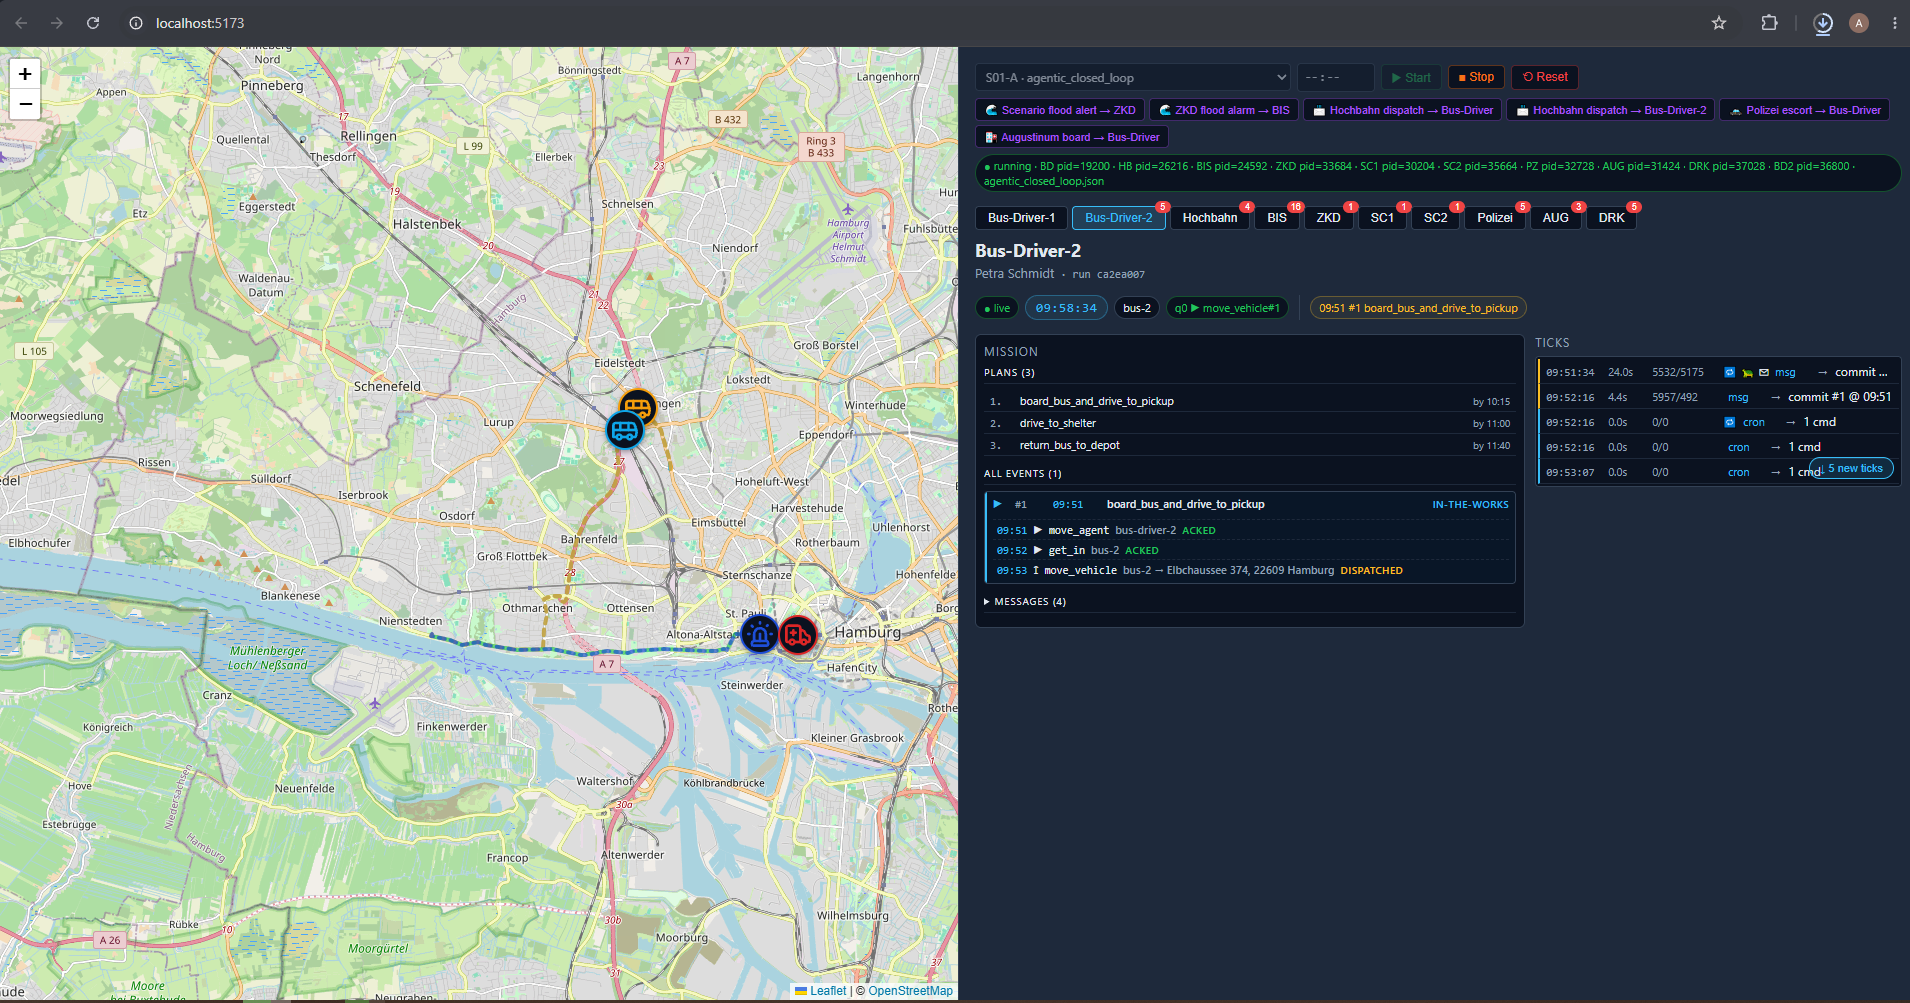
\includegraphics[width=0.92\textwidth,height=0.72\textheight,keepaspectratio]{ui-main.png}
  \par\medskip
  \small We can watch a live agentic run on the map, and open the full
  prompt and answer behind any single decision.
  \note{The baseline has no live view. The tick drawer is in the backup
  slides if someone asks how we know what the model was thinking.}
\end{frame}

% =====================================================================
\section{Method}

\begin{frame}{Evaluation: three gates, read in order}
  \begin{columns}[c,onlytextwidth]
    \column{0.58\textwidth}
      \thesisfig[0.86\textheight]{../pics/method-gates}
    \column{0.39\textwidth}
      \small
      \begin{itemize}
        \item 7 scenarios, $k = 10$ paired runs per cell, common random
          numbers.
        \item 310 scored runs. Three models completed the novel arm:
          glm-5.2, deepseek-v4-pro, qwen3.5.
        \item Pre-registered: $\delta_{NI} = 0.05$ on survival,
          $\delta_m = 1$ whole level.
        \item Four hypotheses. H1 and H2 are confirmatory.
        \item The third model slot changed after data were seen, so the
          novel-arm model set is exploratory.
      \end{itemize}
  \end{columns}
  \note{A system that loses residents has lost, however fast it was.}
\end{frame}

\begin{frame}{What we measure}
  \begin{columns}[c,onlytextwidth]
    \column{0.36\textwidth}
      \[
        S = \frac{\text{valid residents}}{\text{ceiling}}
      \]
    \column{0.60\textwidth}
      Valid means delivered before the deadline, into a shelter within its
      declared beds. The ceiling is 100.
  \end{columns}
  \bigskip
  \thesisfig[0.45\textheight]{figs/method-ladder}
  \medskip
  Every cut has a reason written before the runs: 0.10 is one part-load of
  one bus, 0.50 is half the home. Level 4 also needs the run to drive at
  most 25\,\% further than the same system and model's undisrupted runs.
  \note{One ordinal ladder over valid completeness, every cut justified
  before the runs. Level 4 adds an efficiency check against the system's
  own undisrupted runs.}
\end{frame}

% =====================================================================
\section{Results}

\begin{frame}{RQ1: both confirmatory hypotheses fail}
  \begin{columns}[T,onlytextwidth]
    \column{0.46\textwidth}
      Mean survival on the 50 novel runs per system
      \medskip

      \centering
      \begin{tabular}{lc}
        \toprule
        System / model & mean $S$ \\
        \midrule
        workflow baseline & \textbf{1.000} \\
        agentic / qwen3.5 & 0.894 \\
        agentic / glm-5.2 & 0.840 \\
        agentic / deepseek-v4-pro & 0.727 \\
        \bottomrule
      \end{tabular}
      \par\smallskip
      {\scriptsize qwen3.5 capped at 1.0 per run (three runs scored 1.1).}
    \column{0.50\textwidth}
      \small
      \begin{itemize}
        \item \textbf{Gate~1 fails 26 of 27 cells.} Three are on the road
          closure, which is not like-for-like. Without them, 23 of 24.
        \item \textbf{H1} (non-inferiority, anticipated arm): holds in 1 of
          8 cells, glm-5.2 on the undisrupted \code{closed_loop}.
        \item \textbf{H2} (superiority, novel arm): 0 of 19 cells pass, and
          no cell reaches the one-level minimum effect.
        \item H3 is unresolved. H4 was not tested: every run used one time
          scale.
      \end{itemize}
  \end{columns}
  \note{The baseline sheltered every resident in all 50 novel runs. The one
  pass anywhere is a non-inferiority pass, not a superiority one.}
\end{frame}

\begin{frame}{The baseline wins on all five novel disruptions}
  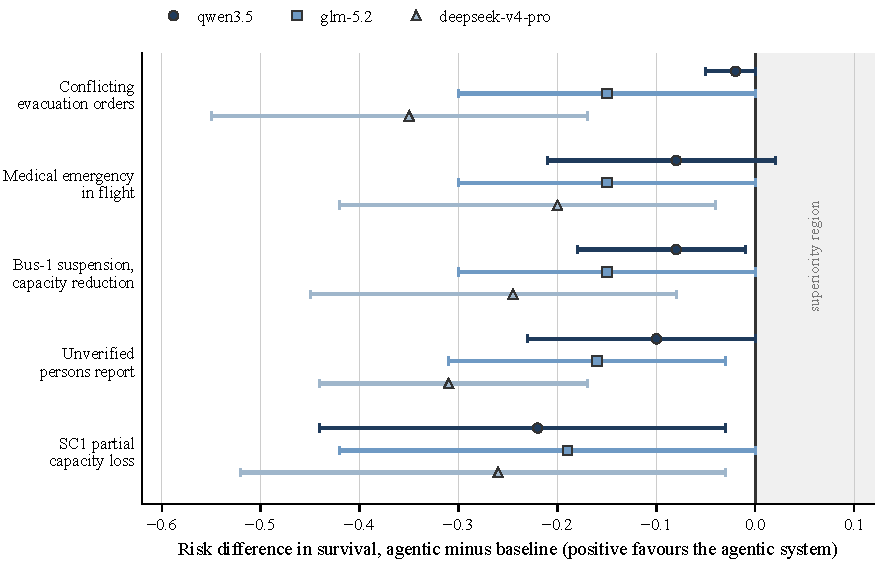
\includegraphics[width=\textwidth,height=0.70\textheight,keepaspectratio]{results-forest-rd.pdf}
  \par\smallskip
  \small Every point estimate is below zero, and no cell shows superiority.
  The gap shrinks with the model: mean risk difference $-0.27$ (deepseek),
  $-0.16$ (glm-5.2), $-0.10$ (qwen3.5).
  \note{Risk difference is agentic minus baseline survival, paired. Do not
  extrapolate past qwen3.5: the design shows no capability threshold.}
\end{frame}

\begin{frame}{RQ2: what we ruled out}
  \small
  Tested against the 150 agentic novel runs. These tests were designed after
  the data were seen, so they are exploratory.
  \medskip

  \begin{tabularx}{\textwidth}{@{}>{\raggedright\arraybackslash}p{6.0cm}>{\raggedright\arraybackslash}X@{}}
    \toprule
    Candidate cause & Verdict \\
    \midrule
    The agents were told the wrong population & No. 100 residents reported in 150 of 150 runs. \\
    The database message layer failed & No. 93.8\,\% of 1,932 addressed requests were answered. \\
    Too few missions dispatched, reserve bus held back & No. About 2.3 dispatch orders in failing and successful runs alike. Bus-2 used in all 150 runs. \\
    The scorer removed real deliveries & No. De-duplicated arrivals track sheltered residents. \\
    Drivers over-claimed their headcount & Does not explain it. An over-report raises $S$. \\
    The run ran out of clock & Mostly no. 5 of the 19 total-loss runs dropped off after 12:00. \\
    \bottomrule
  \end{tabularx}
  \medskip

  What remains is that legs already dispatched were not carried through to
  a drop-off.
  \note{Our first reading under Protocol v1 blamed the handshakes. Protocol v2
  measured them, and closure was 0.938.}
\end{frame}

\begin{frame}{The loss comes in discrete amounts}
  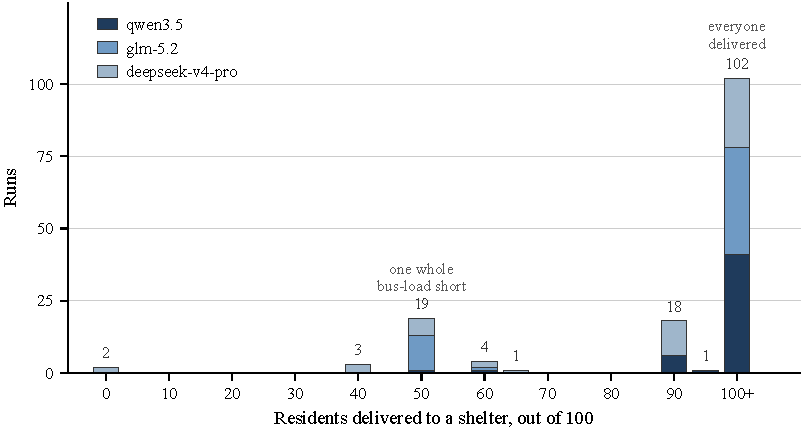
\includegraphics[width=\textwidth,height=0.70\textheight,keepaspectratio]{results-delivery-histogram.pdf}
  \par\smallskip
  \small Of 150 novel runs, 102 delivered everyone, 19 delivered 50 (one
  bus-load short) and 18 delivered 90. A slow loss of quality would spread
  the runs out.
  \note{The spike at 50 matches one bus-load. The spike at 90 matches none,
  so do not call it a bus-load.}
\end{frame}

\begin{frame}{More plan revisions, fewer residents delivered}
  \begin{columns}[c,onlytextwidth]
    \column{0.60\textwidth}
      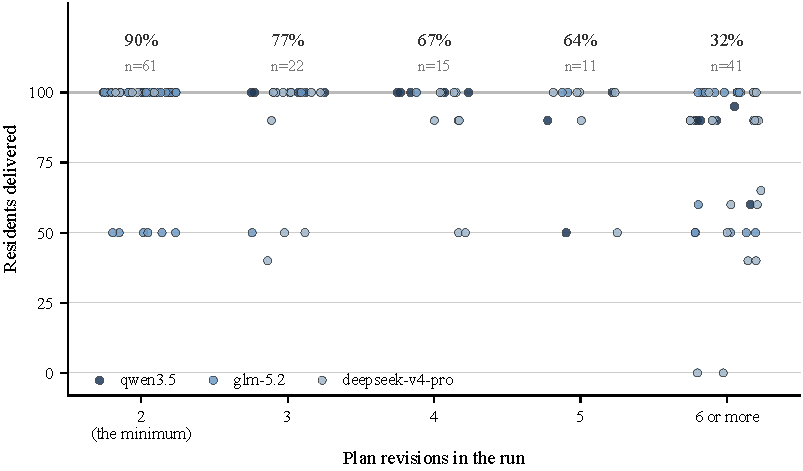
\includegraphics[width=\linewidth]{results-commitment-scatter.pdf}
    \column{0.37\textwidth}
      \small
      Full delivery falls from \textbf{90\,\%} at the fewest revisions to
      \textbf{32\,\%} at six or more.
      \medskip

      \begin{block}{Leading hypothesis: a commitment failure}
        \footnotesize
        \begin{itemize}
          \item Comprehension was not measured.
          \item Causal direction is open: 57 of 108 aborts are stand-downs
            after a failure.
          \item Live field agents against a simulator (deviation~7): we
            cannot separate command post from field.
        \end{itemize}
      \end{block}
  \end{columns}
  \note{An intention is a plan the agent keeps until it has a reason to drop
  it (Rao and Georgeff). On these scenarios the correct number of re-plans was
  zero.}
\end{frame}

\begin{frame}{Decision quality is split}
  \begin{columns}[c,onlytextwidth]
    \column{0.58\textwidth}
      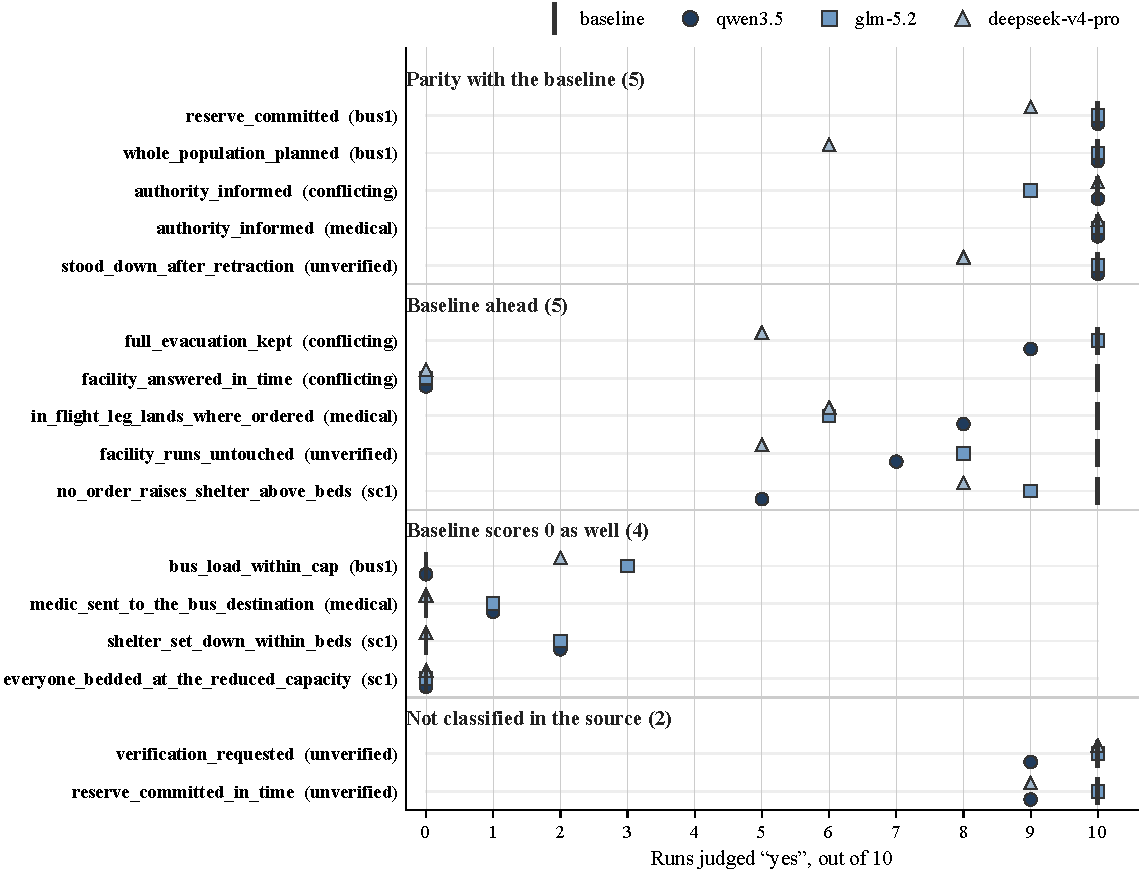
\includegraphics[width=\linewidth,height=0.86\textheight,keepaspectratio]{results-rubric-split.pdf}
    \column{0.39\textwidth}
      \small
      16 held-out rubric criteria, checked on the event log and fixed
      before the novel runs.
      \begin{itemize}
        \item \textbf{Parity on 5}, all about deciding: inform the
          authority, commit the reserve, plan for everyone.
        \item \textbf{Baseline ahead on 5}, mostly about closing the loop.
        \item \code{facility_answered_in_time}: baseline 10 of 10, every
          agentic model 0.
        \item On 4 more the baseline also scores 0.
      \end{itemize}
  \end{columns}
  \note{Use this slide whenever someone rounds the result to
  decision-quality parity. It is split.}
\end{frame}

\begin{frame}{The test could not be lost}
  \begin{columns}[T,onlytextwidth]
    \column{0.42\textwidth}
      \small
      A no-replan control ignores every disruption. On all five novel
      scenarios it commits byte-identical orders, drives the same 60.63
      bus-km and reaches the same level as the baseline.
      \medskip

      \begin{itemize}
        \item The baseline's $S = 1.000$ is the null policy's score, so it
          says nothing about adaptation.
        \item Gate~0 admits 0 of the 6 disruption scenarios.
        \item The agentic system is below doing nothing in all 15 novel
          cells, and in 68 of 150 runs.
        \item Part of the gap exists undisrupted: \code{closed_loop}
          $S$ is 1.000 (glm), 0.950 (qwen3.5), 0.790 (deepseek).
      \end{itemize}
    \column{0.55\textwidth}
      \vspace{6mm}
      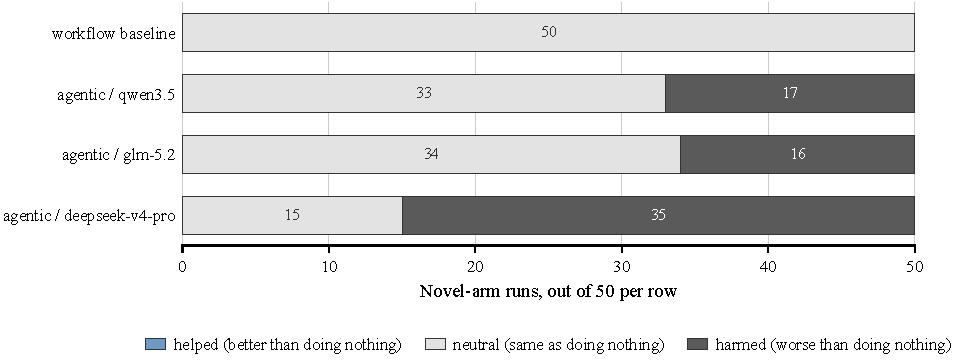
\includegraphics[width=\linewidth]{critique-regret.pdf}
  \end{columns}
  \note{The protocol found with its own negative control that its primary
  arm could not resolve H2. Say ``below doing nothing'', never that the
  system harmed itself by responding.}
\end{frame}

\begin{frame}{What the agentic approach costs}
  \centering
  \small
  \begin{tabular}{lcccc}
    \toprule
    System / model & messages & msgs / resident & tokens & budget fraction \\
    \midrule
    workflow baseline & 13.2 & \textbf{0.13} & 0 & 0.00 \\
    agentic / deepseek-v4-pro & 91.9 & 1.26 & 725,457 & 1.80 \\
    agentic / qwen3.5 & 106.6 & 1.18 & 894,243 & 2.28 \\
    agentic / glm-5.2 & 111.8 & 1.33 & 829,906 & 2.70 \\
    \bottomrule
  \end{tabular}
  \par\bigskip
  \raggedright
  \begin{itemize}
    \item Nine to ten times the baseline's messages per resident delivered.
    \item 140 of 150 agentic novel runs finished over the time budget.
    \item The baseline is deterministic and calls no model.
  \end{itemize}
  \note{The baseline wins on speed and cost, and it also won the primary
  outcome. On these scenarios the cost bought no survival.}
\end{frame}

% =====================================================================
\section{Design considerations}

\begin{frame}{RQ3: what a designer should consider}
  \small
  \begin{tabularx}{\textwidth}{@{}>{\raggedright\arraybackslash}X>{\raggedright\arraybackslash}p{3.9cm}@{}}
    \toprule
    Consideration & Measured in this study \\
    \midrule
    \textbf{1. Commit, then confirm.} A leg on the road stays committed
      unless the agent states a reason, and the runtime counts it. Every leg
      gets an explicit delivery confirmation.
      & Full delivery 90\,\% $\to$ 32\,\% as plan revisions rise \\
    \addlinespace
    \textbf{2. Make the problem real.} A disruption must change the state
      the scorer reads. SC1 was reported at 40 beds and still declared 60.
      & Orders byte-identical to the no-replan control \\
    \addlinespace
    \textbf{3. Test the test first.} Run Gate~0 before the campaign, size
      the design before the runs, fix and pin the models.
      & Sign test cannot go below $p = 0.0625$ at 5 scenarios \\
    \addlinespace
    \textbf{4. Plan the cost.} Decide what the extra messages and tokens
      have to buy.
      & 9 to 10 times the messages per resident \\
    \bottomrule
  \end{tabularx}

  \medskip
  These come from one evaluation of one architecture on one case. The
  commitment boundary rests on an association, not yet on a cause.
  \note{Each consideration is tied to one measurement in this study.}
\end{frame}

% =====================================================================
\section{Conclusion}

\begin{frame}{Contributions}
  \begin{enumerate}
    \item \textbf{An agentic architecture and its baseline.} Ten agents
      coordinating through PostgreSQL, and a DV~100 baseline that shares
      the scenarios, actions and scoring.
    \item \textbf{A scored comparison with a negative result.} 310 runs,
      seven scenarios, pre-registered hypotheses, deterministic scoring.
    \item \textbf{A diagnosis of the loss.} Messages worked. Dispatched legs
      were not carried through. Leading hypothesis: commitment.
    \item \textbf{A method for a fair comparison.} A shared append-only
      event log, regret against a null policy, and Gate~0 as a check on
      treatment validity.
  \end{enumerate}
  \note{The method can be reused without our architecture.}
\end{frame}

\begin{frame}{Conclusion}
  \begin{block}{Answers}
    \begin{description}[RQ1]
      \item[RQ1] On our scenarios, no. The baseline won on all five novel
        disruptions, and the agentic system scored below doing nothing.
        Whether it can ever win remains open.
      \item[RQ2] Messages worked and missions were dispatched. Committed legs
        were not carried through to delivery. Leading hypothesis: a failure
        of commitment.
      \item[RQ3] Commit, then confirm. Make disruptions change the world.
        Pass Gate~0 first. Plan the cost.
    \end{description}
  \end{block}
  \begin{exampleblock}{Next experiment}
    A commitment-constrained variant on the same scenarios and models. If it
    delivers more, plan churn is a cause. If not, churn is a symptom. Then
    scenarios that pass Gate~0.
  \end{exampleblock}
  \note{We expected LLM agents to handle disruptions that a script did not
  foresee. On the disruptions we tested, the script delivered every resident
  in every run, and the agents did not.}
\end{frame}

\begin{frame}[standout]
  Thank you.\\[6pt]
  Questions?
\end{frame}

% =====================================================================
\appendix

\begin{frame}{Backup: the seven parity deviations}
  \scriptsize
  \begin{tabularx}{\textwidth}{c>{\raggedright\arraybackslash}X>{\raggedright\arraybackslash}p{4.6cm}}
    \toprule
    \# & Deviation & Effect on a result \\
    \midrule
    1 & A baseline message's id is its position in the run, not a clock time. & None. No code reads it. \\
    2 & A baseline message names its receiver. & None. No code reads it. \\
    3 & A baseline record is labelled as a decision. & None. Scored facts do not change. \\
    4 & A baseline record has an empty model name. & None. The scorer reads no model name. \\
    5 & One node, the IC, holds the command and the fleet picture. & Favours the baseline. This is the doctrine. \\
    6 & The IC plans its schedule with road distance and travel time. & Favours the baseline. \\
    7 & Only the baseline's scenario files declare a world. A simulator carries out the IC's orders; the agentic side runs its field agents live. & Mixed. No scripted drop-offs: against the baseline. Simulator in place of live agents: for it. \\
    \bottomrule
  \end{tabularx}
  \note{Deviation 7 cuts both ways, which is why RQ2 cannot separate the
  command post from the field agents.}
\end{frame}

\begin{frame}{Backup: risk differences per novel cell}
  \small
  $RD = S_\text{agentic} - S_\text{baseline}$, paired, with 95\,\% CI.
  \medskip

  \centering\footnotesize
  \begin{tabular}{lccc}
    \toprule
    Disruption & qwen3.5 & glm-5.2 & deepseek-v4-pro \\
    \midrule
    Conflicting evacuation orders & $-0.02$ [$-0.05$, 0.00] & $-0.15$ [$-0.30$, 0.00] & $-0.35$ [$-0.55$, $-0.17$] \\
    Medical emergency in flight & $-0.08$ [$-0.21$, 0.02] & $-0.15$ [$-0.30$, 0.00] & $-0.20$ [$-0.42$, $-0.04$] \\
    Reduced bus capacity & $-0.08$ [$-0.18$, $-0.01$] & $-0.15$ [$-0.30$, 0.00] & $-0.245$ [$-0.45$, $-0.08$] \\
    Unverified persons report & $-0.10$ [$-0.23$, 0.00] & $-0.16$ [$-0.31$, $-0.03$] & $-0.31$ [$-0.44$, $-0.17$] \\
    SC1 partial capacity loss & $-0.22$ [$-0.44$, $-0.03$] & $-0.19$ [$-0.42$, 0.00] & $-0.26$ [$-0.52$, $-0.03$] \\
    \bottomrule
  \end{tabular}
\end{frame}

\begin{frame}{Backup: anticipated arm}
  \centering
  \begin{tabular}{lcc}
    \toprule
    System / model & \code{closed_loop} & \code{road_closure} \\
    \midrule
    workflow baseline & 1.000 & 0.60 against the nominal 100 \\
    agentic / glm-5.2 & 1.000 (H1 pass) & 0.84 \\
    agentic / qwen3.5 & 0.950 & not run \\
    agentic / deepseek-v4-pro & 0.790 & 0.70 \\
    \bottomrule
  \end{tabular}
  \par\bigskip
  \raggedright\small
  On the road closure the baseline's file makes one school unreachable and
  declares 60 residents, while the agentic file has 100 and a detour. The two
  systems ran different scenarios there.
\end{frame}

\begin{frame}{Backup: Gate~0 evidence}
  \scriptsize
  \centering
  \begin{tabular}{lccccccc}
    \toprule
     & & orders & \multicolumn{2}{c}{level $L$ (C)} & \multicolumn{2}{c}{bus-km} & discri- \\
    \cmidrule(lr){4-5}\cmidrule(lr){6-7}
    Scenario & world & identical & doctrine & no-replan & doctrine & no-replan & minates \\
    \midrule
    \emph{fixture:} \code{shelter_closure} & yes & no & 3 (1.0) & 0 (0.0) & 83.12 & 38.14 & \textbf{yes} \\
    \midrule
    \code{medical_emergency_in_flight} & yes & yes & 3 (1.0) & 3 (1.0) & 60.63 & 60.63 & no \\
    \code{unverified_persons_report} & yes & yes & 3 (1.0) & 3 (1.0) & 60.63 & 60.63 & no \\
    \code{conflicting_evacuation_orders} & yes & yes & 3 (1.0) & 3 (1.0) & 60.63 & 60.63 & no \\
    \code{bus1_suspension_capacity_reduction} & yes & yes & 3 (1.0) & 3 (1.0) & 60.63 & 60.63 & no \\
    \code{sc1_partial_capacity_loss} & yes & yes & 3 (1.0) & 3 (1.0) & 60.63 & 60.63 & no \\
    \code{closed_loop} & yes & yes & 3 (1.0) & 3 (1.0) & 60.63 & 60.63 & no \\
    \code{road_closure} & no & no & 3 (1.0) & 3 (1.0) & 83.12 & 38.14 & no \\
    \bottomrule
  \end{tabular}
  \par\medskip
  \raggedright\small
  Level capped at 3 here. Only the shelter-closure fixture discriminates.
\end{frame}

\begin{frame}{Backup: why the registered H2 primary could not decide}
  \small
  \begin{itemize}
    \item Registered primary: a Clopper--Pearson interval on
      $P(L_\text{agentic} \geq L_\text{baseline})$ per cell, a sign test
      across scenarios, Holm--Bonferroni. Implemented after the data were
      seen (Amendment 15).
    \item It agrees with the risk difference: no cell is above chance.
    \item At $k = 10$ every interval is about 0.6 wide.
    \item A two-sided exact sign test over five scenarios cannot return less
      than $p = 0.0625$. With two ties the floor is 0.250, and qwen3.5 and
      glm-5.2 sit on it.
  \end{itemize}
  \medskip
  The risk difference, continuous and paired, carries the argument.
\end{frame}

\begin{frame}{Backup: the twelve tables}
  \thesisfig[0.86\textheight]{../pics/data-tables}
\end{frame}

\begin{frame}{Backup: inside one decision}
  \centering
  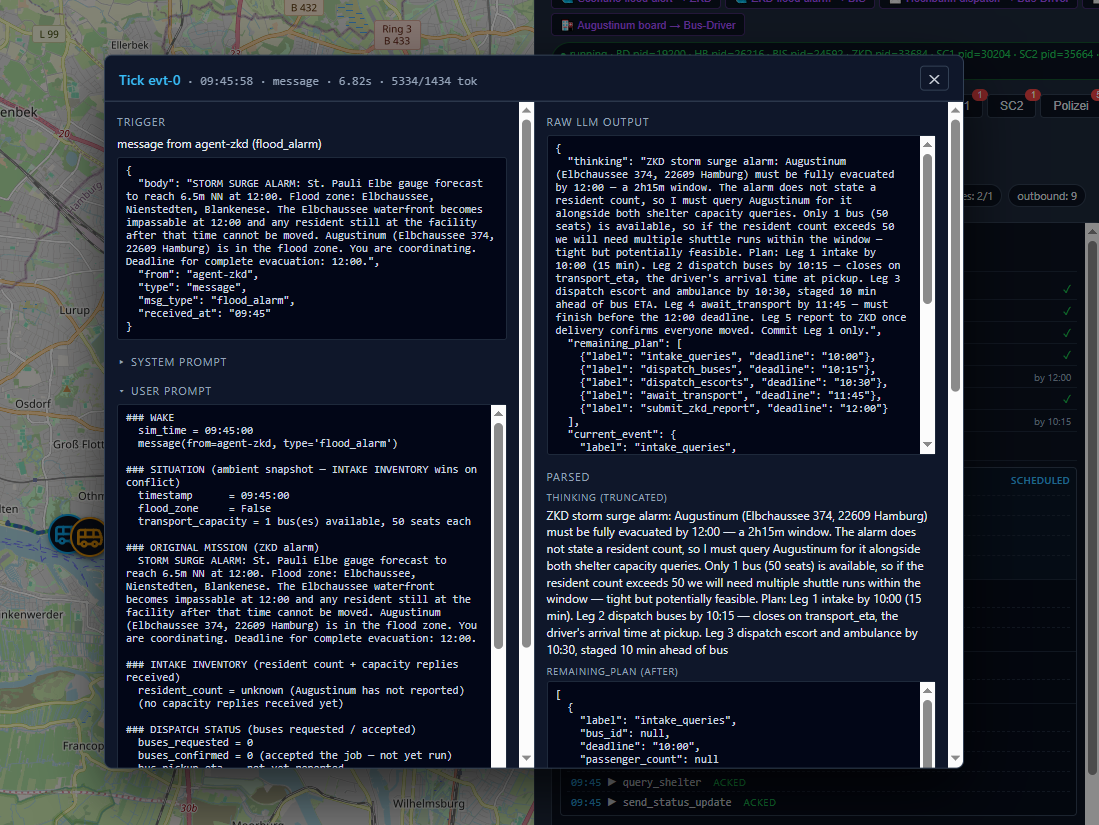
\includegraphics[width=\textwidth,height=0.72\textheight,keepaspectratio]{ui-tick-drawer.png}
  \par\smallskip
  \small BIS woken by the storm surge alarm: the prompt on the left, the raw
  model output and the parsed plan on the right.
\end{frame}

\begin{frame}{Backup: how the interface reads the database}
  \thesisfig[0.86\textheight]{../pics/ui-dataflow}
\end{frame}

\begin{frame}[allowframebreaks]{References}
  \printbibliography[heading=none]
\end{frame}

\end{document}
